\documentclass{fiwthesis}
%\documentclass[en]{fiwthesis}   % Default language is german but can be switched to english

% ========
%  Pakete
% ========

\usepackage{textgreek}           % griechische Buchstaben außerhalb des Math-Mode
\usepackage{amsmath}             % zentrierte Formeln
\usepackage{amssymb}             % erweiterter Formelsatz mathem. Symbole

\usepackage{boldline}            % breitere Linien in Tabellen
\usepackage{booktabs}            % typographisch richtige Tabellen setzen
\usepackage{tabularx}            % Erweiterte Tabellendarstellung
\usepackage{multirow}            % Spalte über mehrere Zeilen oder Spalten ausdehnen
\usepackage{xltabular}           % Zeilenumbrüche in tabularx erlauben

\usepackage{graphicx}            % ermöglicht das Einbinden von Grafiken
\usepackage{subcaption}          % mehrere Bilder in einem Bild
\usepackage{pgfplots}            % Grafiken erzeugen
\usepackage{smartdiagram}        % schnelle und einfache Grafiken
\usepackage{pdfpages}            % Einbinden von PDFs
\usepackage{orcidlink}           % ORCID ID einbinden
\usepackage{makecell}            % Tabellenzellen formatieren
\usepackage{hologo}              % LaTeX-Logos setzen
\usepackage{svg}                 % SVG-Grafiken einbinden
\usetikzlibrary{positioning}     % bessere Ortsbezeichnung
\usetikzlibrary{shapes}          % typische Formen wie Rechtecke, Ellipsen usw. einfach zeichnen
\usetikzlibrary{intersections}   % Schnittpunkt von Geraden adressieren
\usetikzlibrary{angles, quotes}  % einfacheres Zeichnen von Winkeln
\usetikzlibrary{                 % Symbole für Schaltpläne
  circuits.logic.US,
  circuits.logic.IEC,
  circuits.logic.CDH,
  circuits.ee.IEC
}

\usepackage{lipsum}

% ===========
%  Metadaten
% ===========

\thesis{Master-Thesis}
\title{Identifikation und Vergleich von Autorenangaben zu Software zwischen verschiedenen Datenquellen}
\author{Kevin Jahrens}
\date{\today}
\matrnr{480592}
\bdate{05.08.1999}
\bcity{Bad Oldesloe}
\supervisor{\makecell[tl]{Prof.~Dr.~-Ing.~Frank Krüger\orcidlink{0000-0002-7925-3363} \\ Hochschule Wismar, Fakultät für Ingenieurwissenschaften \\ Bereich Elektrotechnik und Informatik, Wismar, Deutschland}}
\secsupervisor{\makecell[tl]{M.A.~Stephan Druskat\orcidlink{0000-0003-4925-7248} \\ Deutsches Zentrum für Luft- und Raumfahrt (DLR), \\ Institut für Softwaretechnologie, Berlin, Deutschland}}
\keywords{Data, Science, Software, Author, Comparison, Identification}

% Metadaten in die PDF-Datei schreiben
\makepdfmetadata

% ==========
%  Präambel
% ==========

% PGF Kompatibilitätseinstellung
\pgfplotsset{width=0.95\textwidth,compat=newest}

% % Bibliographie einbinden
\bibliography{quellen}

% Abkürzungen einbinden
%\gls{}         normal zu nutzen (erstes Mal: 'lange Form (kurze Form)'), danach nur 'kurze Form'
%\glspl{}       wie \gls{} nur als Plural
%\acrfull{qrc}  gibt volle Form ('lange Form (kurze Form)') egal wo
%\acrlong{qrc}  gibt lange Form ('lange Form') egal wo
%
%\newacronym{tag}{short}{long}
\newacronym{cff}{CFF}{Citation File Format}
\newacronym{pep}{PEP}{Python Enhancement Proposal}
\newacronym{pypi}{PyPI}{Python Package Index}
\newacronym{cran}{CRAN}{Comprehensive R Archive Network}
\newacronym{ner}{NER}{Named entity recognition}


% Glossar- und Abkürzungsverzeichniserstellung
\makeglossaries{}

% Index erzeugen
\makeindex[
  intoc=true,
  title=Index,
  columns=2]{}
\indexsetup{headers={\indexname}{\indexname}}

% ===============
%  Eigene Makros
% ===============

\newcommand*{\code}[1]{\texttt{#1}}

% ===============
%  Beginn Thesis
% ===============

% TODO Titel erfüllen komplettes Ergebnis darstellen und erklären über die gesamte Arbeit ein Fazit ziehen was erreicht wurde
% TODO Krüger liebt Visualisierungen davon gerne ein paar rein machen -> vllt. auch die vom Forschungsseminar übernehmen?
% TODO ich kann in der Präsentation nicht davon ausgehen, dass die Arbeit gelesen wurde! Somit muss ich auch den kompletten Kontext rüber bringen und die Ziele und was wir überhaupt machen und warum
% TODO Quellen final durch gehen (DOI benötigt keine URL und kein Zugriffsdatum)
% TODO in Quellen 6 Autoren nennen manchmal wird nur 1 genannt -> Krüger wird z. B. nicht genannt
% TODO muss definitiv in der Arbeit beantwortet werden: "Was muss ich machen, dass ich ein Zitationsfähriger Autor bin?" -> Bzw. "Was muss ich machen, damit ich in der Zitation auftauche?"
% TODO wenn ich Simon die arbeit schicke ihm den Hinweise geben, dass mein Prof grafiken und darstellungen liebt. Er soll mich also darauf hinweisen, wo noch sowas eingebaut werden könnte/ Simon sagen, dass er die Arbeit auch gerne an seine Kollegen/ meinen künftigen Kollegen weiterleiten darf die ist eh öffentlich einsehbar wenn man weiß wo man guckt. Aber ich möchte gerne nur eine PDF mit den Kommentaren haben und nicht 20 von allen :o außerdem würde es mich freuen wenn wir die Arbeit noch etwas ausdünnen
% TODO checken, ob ich bei Zitation von software nicht nur die preferred citation zitiere sondern auch die software an sich

\begin{document}

% ============
%  "Vorspann"
% ============

% Titelseite
\maketitle

% Aufgabenstellung
\includepdf[pages=-]{anlagen/aufgabenstellung_print.pdf}

% Abstract
\makeabstract{
  Maximal eine halbe Seite.
}{
  English Version.
}

% Inhaltsverzeichnis (Schalter `compact' sorgt für einfachen Zeilenabstand)
\maketoc[compact]

% ==========
%  Textteil
% ==========

\newcolumntype{P}[1]{>{\centering\arraybackslash}p{#1}}
\newcolumntype{L}[1]{>{\raggedright\arraybackslash}p{#1}}
\newcolumntype{R}[1]{>{\raggedleft\arraybackslash}p{#1}}

\setlength{\belowcaptionskip}{\baselineskip}

% Einleitung
\chapter{Einleitung}
\label{chap:einleitung}
\section{Motivation}
\label{sec:motivation}
\section{Vorgehen}
\label{sec:vorgehen}
\section{Gliederung}
\label{sec:gliederung}


% weitere Kapitel hier jeweils einzeln einbinden
\chapter{Grundlagen}
\label{chap:grundlagen}
% TODO Auf Zenodo eingehen? Checken was das ist
\section{Zitation von Software}
\label{sec:software-zitation}
% TODO Irgendwo auf die Sachen eingehen: https://github.com/citation-file-format/citation-file-format/blob/main/schema-guide.md#preferred-citation
% TODO https://peerj.com/articles/cs-86/
% TODO auf notwendigkeit von Software Zitation eingehen und warum Zitation von Software wichtig ist
% TODO Auch Zitation von Personen, welche nicht aktiv an der Software entwickeln (All Contributors)

\section{Versionsverwaltung}
\label{sec:versionsverwaltung}
Die Versionsverwaltung ist ein System, um verschiedene Versionen von Software zu verwalten.
Es bietet Zugang zu Code und dessen Änderungen in der Vergangenheit.
Der Code und getätigte Änderungen werden in einem Repository gespeichert.
Dadurch ist die Versionsverwaltung eine Art Logbuch, in dem alle Änderungen festgehalten werden.
Dabei wird zusätzlich zu der Änderung der Autor und der Zeitpunkt der Änderung festgehalten \autocite{ponuthorai_version_2022}.
Dies ermöglicht es in der Masterarbeit empirisch die Menge an Arbeit der einzelnen Autoren zu ermitteln.

Zusätzlich zum Code können in einem Repository andere Dateien, wie beispielsweise eine README, eine Lizenz, und Zitationsinformationen, beispielsweise in Form einer \gls{cff}-Datei, gespeichert werden.
Eine README-Datei ist eine Datei, welche Informationen über das Projekt enthält, beispielsweise wie es installiert und verwendet wird.
Sie wird standardmäßig im Stammverzeichnis des Repositorys gespeichert und wird an dieser Stelle auch von Diensten wie GitHub dargestellt.

Es gibt zwei verschiedene Arten von Versionsverwaltungssystemen.
Zum einen gibt es die zentralen Systeme, bei denen alle Änderungen zentral verwaltet werden, beispielsweise SVN.
Zum anderen gibt es die verteilten Systeme, bei denen jeder Entwickler eine Kopie des gesamten Repositorys und dessen Vergangenheit hat \autocite{ponuthorai_version_2022}.
Ein solches System ist Git, welches sich mit einem Marktanteil von ungefähr 75 \% gegenüber anderen Systemen durchgesetzt hat \autocite{lindner_version_2024}.
Aus diesem Grund und weil Git-Repositorys in der Arbeit untersucht werden, wird auf Git eingegangen.
Dabei werden Begriffe erklärt, mit denen es möglich ist, die geleistete Arbeit von einzelnen Autoren innerhalb eines Repositorys zu untersuchen.
Außerdem wird auf grundlegende Funktionen von Git eingegangen, da diese für die Arbeit relevant sind.
Der Aufbau der einzelnen Git-Komponenten ist in \autoref{fig:git} dargestellt.
Dabei ist zu erkennen, dass Git in einen Git-Server und Git-Anwendungen aufgeteilt wurde.

\begin{figure}
    {   
        \begin{center}
            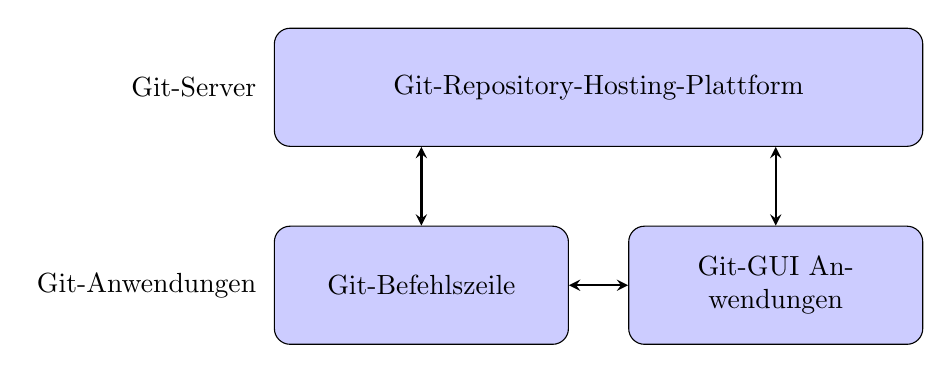
\begin{tikzpicture}
                [
                    block/.style = {rectangle, draw, fill=blue!20, text width=8cm, text centered, minimum height=1.5cm, rounded corners=0.2cm},
                    client/.style = {rectangle, draw, fill=blue!20, text width=3.5cm, text centered, minimum height=1.5cm, rounded corners=0.2cm},
                    arrow/.style = {thick,<->,>=stealth}
                ]
        
                \node (server) [block] {Git-Repository-Hosting-Plattform};
                \node (cli) [client, below=of server, xshift=-2.25cm] {Git-Befehlszeile};
                \node (gui) [client, below=of server, xshift=+2.25cm] {Git-GUI Anwendungen};
            
                \draw[arrow] (cli.north) -- (server.south -| cli.north);
                \draw[arrow] (gui.north) -- (server.south -| gui.north);
                \draw[arrow] (cli) -- (gui);

                \node[left=0.1cm of server] {Git-Server};
                \node[left=0.1cm of cli] {Git-Anwendungen};
            
            \end{tikzpicture}
        \end{center}
        \caption{Übersicht über die Git-Komponenten}
        \label{fig:git}
        \small
        Die Git-Komponenten bestehen aus einem Git-Server, welcher das Repository hostet, und Git-Anwendungen, welche auf das Repository zugreifen (indirekt aus \cite{ponuthorai_version_2022}).
    }
\end{figure}

Bei der Benutzung von Git ist ein Server nicht zwingend erforderlich, jedoch steigert dies die Komplexität der Verwaltung und ist komplizierter in der Handhabung.
Der Git-Server ermöglicht die einfache kollaborative Entwicklung von Code, da dieser ständig erreichbar ist und zentral verwaltet wird \autocite{ponuthorai_version_2022}.
Standardmäßig wird auf dem Git-Server die neueste Version des Repositorys gespeichert.
Ein möglicher Git-Server ist GitHub, auf welchen im späteren Verlauf weiter eingegangen wird.
Git-Anwendungen sind Programme, welche mit dem lokalen Repository interagieren \autocite{ponuthorai_version_2022}.
Diese können auf entfernte Git-Repositorys zugreifen, wie beispielsweise Repositorys, welche auf GitHub gehostet werden.
Anschließend arbeiten die Programme auf der lokalen Kopie und können die Änderungen, wenn nötig, auf das entfernte Repository übertragen.

In Repositorys werden verschiedene Arten von Statistiken gespeichert.
Git verwaltet Revisionen als \emph{Snapshot}.
Anders als in anderen Systemen wird keine Serie von Änderungen gespeichert, sondern ein \emph{Snapshot} der Änderungen zu einem bestimmten Zeitpunkt erstellt \autocite{ponuthorai_version_2022}.
Dies wird ein Commit genannt.
An einem Commit werden verschiedene Metainformationen gespeichert, beispielsweise eine Commit-Nachricht, der Autor und der Zeitpunkt der Änderungen.

Die Änderung wird dabei als zwei Zeitpunkte angegeben.
Zum einen wird der Zeitpunkt der Änderung des Autors angegeben, also jener Zeitpunkt, zu dem der Autor die Änderung vorgenommen und committet hat, dies wird in Git \emph{author date} genannt.
Zum anderen wird der Zeitpunkt des Einfügens des Commits in das Repository gespeichert, dies wird in Git \emph{commit date} genannt.
Der Commit kann von einer anderen Person, z. B. durch einen Projektverantwortlichen, mittels eines Pull Requests in das Repository übernommen worden sein.
Durch dieses Verhältnis ist der \emph{commit date} Zeitpunkt immer später oder gleich dem \emph{author date} Zeitpunkt.
Außerdem ist gewährleistet, dass beide verantwortlichen Anerkennung für die geleistete Arbeit erhalten \autocite{chacon_pro_2024}.

Die Commit-Nachricht, sowie der Autor mit E-Mail-Adresse und Namen können in den Einstellungen von Git frei gewählt werden, müssen jedoch vorhanden sein, um einen Commit erstellen zu können.
Mehrere Commits bilden die Commit-Historie bzw. die Vergangenheit eines Repositorys.
Weitere Eigenschaften, welche sich aus dem Repository exportieren lassen, sind die Anzahl der eingefügten und gelöschten Zeilen.
Zudem lässt sich die Anzahl der geänderten Dateien ermitteln.
Diese Werte können für das gesamte Repository oder für einzelne Autoren ermittelt werden.

Ein Repository kann verschiedene Branches enthalten, muss jedoch mindestens einen enthalten.
In der Vergangenheit wurde der Standardbranch \emph{master} genannt.
Seit 2020 wird dieser jedoch in \emph{main} umbenannt, um rassistische Konnotationen zu vermeiden \autocite{github_githubrenaming_2024}.
Ein Branch ist eine separate Entwicklungslinie, welche unabhängig von anderen Branches ist.
Beim Erstellen von einem Branch wird der aktuelle Zustand des Branches, auf welchem der neue Branch erstellt wird, kopiert \autocite{ponuthorai_version_2022}.
Dadurch können Änderungen in dem neuen Branch durchgeführt werden, ohne dass diese Änderungen den ursprünglichen Branch beeinflussen.
Diese Änderungen werden mittels Commits festgehalten.
Unterschiedliche Branches können anschließend zusammengeführt werden, um die Änderungen in einem Branch in einen anderen Branch zu übernehmen.

Die Statistiken der Repositorys können auf verschiedene Arten aufgearbeitet werden.
Zum einen können einige direkt mittels Git-Befehlen ausgelesen werden \autocite{chacon_git_2024}.
Andere wiederum benötigen komplexere Abfragen, welche beispielsweise mittels Skripten oder speziellen Programmen ausgelesen werden können.
Ein Beispiel für ein Programm, welches Git-Statistiken aufarbeitet, ist \emph{git-quick-stats} \autocite{mestan_git-quick-stats_2024}.
Außerdem bieten Onlinedienste zur Versionsverwaltung, wie GitHub, Statistiken über APIs an, welche jedoch im Umfang der Anfragen limitiert sind \autocite{github_rate_2022}.
Bei der Benutzung der API von GitHub zum Abfragen der Autoren eines Repositorys werden automatisch alle E-Mail-Adressen der Autoren in Git mit den E-Mail-Adressen, welche die Autoren in GitHub angegeben haben, abgeglichen \autocite{github_rest-api-endpunkte_2022}.
Dadurch werden die Autoren eindeutig zugeordnet und deren Commits addiert.
Diese Werte werden ebenfalls in der Weboberfläche von GitHub angezeigt.

GitHub ist eine Plattform, auf welcher Git-Repositorys gehostet werden können und dient somit als ein Git-Server.
GitHub bietet zusätzliche Funktionen an, welche über die Standardfunktionen von Git hinausgehen.
Diese umfassen unter anderem die kollaborative Entwicklung von Code, Automatisation mittels CI/CD, Sicherheitsaspekte, Projektmanagement, Team Administration und Client-Anwendungen zur Verwaltung von Repositorys \autocite{ponuthorai_version_2022}.
Aktuell benutzen GitHub über 100 Millionen Entwickler und mehr als 4 Millionen Organisationen.
Insgesamt verwaltet die Plattform über 420 Millionen Repositorys.
Außerdem ist GitHub in 90 \% der Fortune 100 Unternehmen im Einsatz \autocite{github_about_2024}.
Um die zusätzlichen Funktionen von GitHub bereitzustellen, werden sogenannte Issues, Pull Requests, geschützte Branches, Actions, Diskussionen und Wikis eingesetzt.
GitHub-Issues sind eine Möglichkeit, um Probleme und Aufgaben zu verfolgen.
Pull Requests dienen dazu, Änderungen in einem Branch eines Repositorys anzufragen und über diese zu informieren.
In dem Pull Requests kann der Code überprüft und diskutiert werden.

\section{Paketverwaltung}
\label{sec:paketverwaltung}

\section{Zitationsformate}
\label{sec:zitationsformate}
\subsection{Citation File Format}
\label{subsec:citation-file-format}
\subsection{BibTeX}
\label{subsec:bibtex_format}

\section{Named Entity Recognition}
\label{sec:named-entity-recognition}

\section{Author name disambiguation}
\label{sec:author-name-disambiguation}
% TODO auf Entity Resolution oder Author name disambiguation eingehen?

\section{Fuzzy Suche}
\label{sec:fuzzy}


\chapter{Methodik}
\label{chap:methodik}
In diesem Kapitel wird beschrieben, wie die Daten der einzelnen Quellen beschafft, abgeglichen und anschließend ausgewertet werden.
Die Datenbeschaffung wird in \autoref{sec:datenbeschaffung}, der Abgleich in \autoref{sec:abgleich} und die Auswertung in \autoref{sec:auswertung} beschrieben.

Die Datenbeschaffung wurde in die einzelnen Quellen untergliedert.
Einige Methoden zur Datenbeschaffung sind dabei ähnlich, worauf im konkreten Fall eingegangen wird.

Der Abgleich findet jeweils zwischen Git und einer weiteren Quelle statt.
Es existiert kein Abgleich zwischen einzelnen Quellen wie den Daten aus \gls{pypi} und der Beschreibung.
Der Abgleich wird in jeder Datenbeschaffung außer der von Git automatisch durchgeführt.
Die Ergebnisse des Abgleichs werden in einer CSV-Datei gespeichert.
Die Datei wird nur erstellt, falls mindestens ein Eintrag enthalten ist.
Allgemeine Daten, beispielsweise ob die Quelle valide ist, werden ebenfalls in einer CSV-Datei gespeichert.
Falls in einer Quelle keine Daten vorhanden sind, wird keine CSV-Datei für diese erstellt.

Sämtliche Ergebnisse werden, falls verfügbar, zu verschiedenen Zeitpunkten in denen Änderungen an der Quelle vorgenommen wurden ermittelt und gespeichert.
Falls aus der Quelle verschiedene Zeitpunkte der Änderungen vorliegen, wird der Abgleich mit Git jeweils mit der neuesten Version durchgeführt und mit der Version, welche zu dem Zeitpunkt der Änderung in der Quelle vorhanden war.
Dadurch entstehen für ein Paket mehrere Dateien, welche unterschiedliche Werte enthalten.
Es entsteht die in \autoref{fig:datenbeschaffung_ergebnisse} dargestellte Ordnerstruktur, welche die Ergebnisse der Datenbeschaffung darstellt.

\begin{figure}
    \dirtree{%
        .1 /\DTcomment{Wurzelverzeichnis}.
        .2 \path{20210819_161452-0400_bib_authors.csv}\DTcomment{\hologo{BibTeX} Autoren abgeglichen mit den Git-Werten zu diesem Zeitpunkt}.
        .2 \path{20210819_161452-0400_bib_authors_new.csv}\DTcomment{\hologo{BibTeX} Autoren abgeglichen mit den Git-Werten zum neuesten Zeitpunkt}.
        .2 \path{20210819_161452-0400_git_contributors.csv}\DTcomment{Git-Autoren bis zu diesem Zeitpunkt}.
        .2 \path{20221010_124020-0400_readme_authors.csv}\DTcomment{Autoren in der Beschreibung abgeglichen mit den Git-Werten zu diesem Zeitpunkt}.
        .2 \path{20221010_124020-0400_readme_authors_new.csv}\DTcomment{Autoren in der Beschreibung abgeglichen mit den Git-Werten zum neuesten Zeitpunkt}.
        .2 \path{20221010_124020-0400_git_contributors.csv}\DTcomment{Git-Autoren bis zu diesem Zeitpunkt}.
        .2 \path{bib.csv}\DTcomment{Allgemeine informationen zur \hologo{BibTeX}-Datei}.
        .2 \path{readme.csv}\DTcomment{Allgemeine Informationen zur Beschreibung}.
        .2 \path{git_contributors.csv}\DTcomment{Git-Autoren zum neuesten Zeitpunkt}.
        .2 \path{pypi_maintainers.csv}\DTcomment{\gls{pypi} Maintainer}.
        .2 \path{python_authors.csv}\DTcomment{In Python angegebene Autoren}.
    }
    \caption{Ergebnisse der Datenbeschaffung}
    \label{fig:datenbeschaffung_ergebnisse}
    \small
    Die Abbildung stellt einen Ausschnitt der CSV-Dateien der Datenbeschaffung dar.
\end{figure}

Der Prozess findet für jedes zu untersuchende Paket statt und ist in \autoref{fig:programmablauf} visualisiert.
Die Pakete stammen aus den Software-Verzeichnissen \gls{pypi} und \gls{cran}.
Die Ergebnisse des Prozesses werden in fünf Ordnern gespeichert jeweils für \gls{pypi}, \gls{cran}, \gls{cff}, \gls{pypi} \gls{cff} und \gls{cran} \gls{cff}.
Diese Ordner bilden die fünf Top-100-Listen, die in \autoref{sec:datenbeschaffung} näher beschrieben sind.
In jedem Ordner sind jeweils Unterordner für die einzelnen Pakete.
Diese Daten werden für die anschließende Auswertung in \autoref{sec:auswertung} verwendet.
In diesem Abschnitt werden die Ergebnisse der Abgleiche analysiert und zusammengefasst, um Aussagen über alle Pakete hinweg zu treffen.
Die Datenbeschaffung, der Abgleich und die Auswertung sind in Python programmiert und verwenden \gls{oss} auf welche in den jeweiligen Abschnitten eingegangen wird.
Der entwickelte Quellcode ist in einem Git-Repository verfügbar \autocite{jahrens_t20240710-softwareauthors-kj_2025}.
Über alle Abschnitte hinweg wird Pandas in der Version 2.2.2 verwendet, um die Tabellen zu erstellen und zu verarbeiten \autocite{the_pandas_development_team_pandas_2024}.

\begin{figure}
    \begin{center}
        \includesvg[width=.95\linewidth,inkscapelatex=false]{bilder/Ablauf.svg}
    \end{center}
    \caption{Visualisierter Prozess}
    \label{fig:programmablauf}
    \small
    In der Abbildung ist der Prozess visualisiert. Die runden Knoten stellen Prozesse dar. Rautenförmige Knoten repräsentieren Software-Verzeichnisse und rechteckige Knoten repräsentieren die einzelnen zu untersuchenden Quellen, in welchen Autoren genannt werden können. Kanten stellen den Informationsfluss dar, wobei die Kantenbeschriftung die jeweiligen Informationen repräsentiert.
\end{figure}

\section{Datenbeschaffung}
\label{sec:datenbeschaffung}
% TODO MEINE SOFTWARE ZITIEREN! Sonst bin ich nicht besser als alle anderen und auch Probleme und Konfiguration darstellen -> steht in dem Paper smith_software_2016 wie zitiert werden soll? \autocite{richardson_beautifulsoup4_2024}
In diesem Abschnitt wird beschrieben wie das Skript zur Datenbeschaffung aus den einzelnen Quellen aufgebaut ist.
Es wird tqdm in der Version 4.66.5 verwendet, um den Fortschritt der Datenbeschaffung anzuzeigen \autocite{costa-luis_tqdm_2024}.
Die Datenbeschaffung wird in die einzelnen Quellen untergliedert.

Aus den Quellen \nameref{subsec:datenbeschaffung_git}, \nameref{subsec:datenbeschaffung_beschreibung}, \nameref{subsec:datenbeschaffung_cff} und \nameref{subsec:datenbeschaffung_bibtex} können zeitliche Informationen extrahiert werden, da diese in Git verwaltet werden.
Aus diesem Grund werden die Daten jeweils zu der Änderung der Quelle gespeichert.
Dabei ist die maximale Anzahl der Änderungen in die Vergangenheit auf 50 beschränkt, um die Laufzeit des Skripts zu begrenzen.

In \nameref{subsec:datenbeschaffung_cran} ist es nicht möglich die Änderungen in der Zeit zu betrachten.
In der \nameref{subsec:datenbeschaffung_pypi} Quelle ist es teilweise möglich die Änderungszeitpunkte zu erhalten, jedoch ist dies mit Kosten verbunden und erfordert eine andere Vorgehensweise als bei den anderen zeitlichen Daten, da diese nicht direkt aus Git extrahiert werden können.
Die beiden Quellen werden aus diesem Grund nur in der neusten Version betrachtet und enthalten keine Änderungshistorie.

\subsection{Git} % 2 Seiten
\label{subsec:datenbeschaffung_git}
% TODO Beschreiben wie die Commits gezählt wurden. -> Mit oder ohne merges?
% TODO email in komplett kleinschreibung umgewandelt anschließend grouby auf email -> kurz erwähnen weil leute frei entscheiden können was sie angeben
Die Git Daten sind die grundlegenden Daten, welche für die weiteren Schritte benötigt werden.
Sämtliche anderen Quellen werden mit den Git Daten über den in \autoref{sec:abgleich} beschriebenen Prozess abgeglichen.
Zu Beginn muss das Repository von GitHub geclont werden, um die Daten Lokal verarbeiten zu können.
Dabei kommt die \gls{oss} GitPython in der Version 3.1.43 zum Einsatz, welches eine Bibliothek für die einfache Interaktion mittels Python und Git Befehlen darstellt \autocite{thiel_gitpython-developersgitpython_2024}.
Für das Clonen wird der Link zum GitHub Repository benötigt, welcher aus der \gls{pypi} oder \gls{cran} Quelle stammt.
Auf diese Quellen wird in dem \autoref{subsec:datenbeschaffung_pypi} und \autoref{subsec:datenbeschaffung_cran} eingegangen.

Die Auswertung des Repositorys wird mit git-quick-stats in der Version 2.3.0 durchgeführt \autocite{arzzen_git-quick-statsgit-quick-stats_2021}.
Git-Quick-stats bietet einfache und effiziente Möglichkeiten um verschiedene Statistiken in einem Git Repository zu ermitteln.
Das Tool wird in dem Python Skript mit dem Befehl \texttt{git-quick-stats -T} aufgerufen, um detaillierte Statistiken zu erhalten.
Ausgegeben wird eine Liste aller Autoren, welche in dem Repository Änderungen vorgenommen haben.
Diese Liste enthält unter anderem den Namen, die E-Mail, die Anzahl der Einfügungen, Löschungen, geänderten Zeilen, Dateien, Commits, sowie den ersten und letzten Commit.
Die Daten werden in der Datei \texttt{git\_contributors.csv} gespeichert.

Außerdem bietet das Tool die Möglichkeit mit der gesetzten Umgebungsvariablen \textit{\_GIT\_UNTIL=}, alle Änderungen nur bis zu einem bestimmten Zeitpunkt zu betrachten.
Diese Funktion wird verwendet, um die Änderungen bis zu der Aktualisierung einer Quelle zu betrachten.
Die Daten werden beispielsweise in der Datei \texttt{20210819\_161452-0400\_git\_contributors.csv} gespeichert, wobei der erste Teil des Dateinamens den konkreten Tag und Uhrzeit mit zugehöriger Zeitzone angibt.
Für die Verarbeitung der Zeiten in unterschiedlichen Zeitzonen wird das Modul pytz in der Version 2024.2 verwendet \autocite{bishop_stub42pytz_2024}.

\subsection{PyPI} % 2 Seiten
\label{subsec:datenbeschaffung_pypi}
% TODO Daten aus PyPi werden benötigt um das GitHub repo zu finden -> sagen, dass die nicht immer vorhanden sind
% TODO erklären warum BigQuery nicht eingesetzt wird aktuell aber dennoch sinnvoll eingesetzt werden könnte bei anderen anforderungen (z.B. liste mit repo links auf github)
% TODO erklären warum die API verwendet wird und nicht nur die TOML beispielsweise ausgelesen wird -> habe ein pypi paket und brauche die GitHub URL
% TODO sagen warum beides also verifizierte Owner und Maintainer sowhl als auch die Daten aus der TOML abgefragt werden -> sind unterschiedliche Leute und werden unterschiedlich angegeben die einen dürfen sachen auf pypi machen die anderen werden in der toml angegeben und dürfen ggf. nichts in pypi machen
% Checken was verifizierte Nutzer im PyPI Universum bedeutet. Sind es nur verifizierte User die z.B. eine E-Mail hinterlegt haben oder sind es Nutzer die an dem Projekt arbeiten und von PyPI verifiziert sind? Falls es mehrwert hat diese Daten ebenfalls automatisch abfragen und auch in der MA beschreiben, was es nun ist und warum es Mehrwert hat oder auch nicht.
% TODO In MA beschreiben, warum oder warum nicht Mehrwert (PyPI Verifizierte Nutzer)
% TODO Sagen warum die Owner nicht berücksichtigt werden hatte dafür auch irgendwo eine Qulle -> es sind immer org.
% TODO erklären, dass ich den Namen des Betreuers brauche und nicht nur den Benutzernamen über die API und wie ich das gelöst habe mit einem WebScraper
% TODO erklären auf welchen branch ich untersuche ist es immer der Github default? oder nehme ich main? oder master? wie wird das entschieden?
% aiohttp==3.10.3, beautifulsoup4==4.12.3, spacy==3.7.6

\subsection{CRAN} % 2 Seiten
\label{subsec:datenbeschaffung_cran}
% TODO Daten aus CRAN werden benötigt um das GitHub repo zu finden -> sagen, dass die nicht immer vorhanden sind
% TODO rpy2==3.5.16, aiohttp==3.10.3

\subsection{Beschreibung} % 2 Seiten
\label{subsec:datenbeschaffung_beschreibung}
% TODO Es werden alle Namen ausgegeben aber auch eben solche, die gar nichts mit dem Paket zu tun haben wie im fall von highr für CRAN: "Provides syntax highlighting for R source Code. Currently it supports LaTeX and HTML output. Source Code of other languages is supported via Andre Simon's highlight package (https://gitlab.com/saalen/highlight)." Es gibt noch weitere Beispiele z.B. in CRAN magrittr -> vllt eher ergebnis?
% spacy==3.7.6

\subsection{Citation File Format} % 2 Seiten
\label{subsec:datenbeschaffung_cff}
% TODO darauf eingehen, dass ich händisch aktuell geprüft habe ob das GH repo in cran oder pypi ist und daraus meine listen gebaut habe. Dies wäre aber auch automatisch möglich aber mit viel Aufwand und man bräuchte google big query für 100 pakete war dieser weg schneller außerdem gibt es auf PyPi mehrere Pakete die auf ein GitHub repo verlinken. Da müsste einiges beachtet werden um das genau zu machen für 100 war dies besser. Falls es für mehr gemacht werden sollte müsste das überdacht werden.
% TODO darauf eingehen wie die CFF geholt und verarbeitet wurde mit stars verknüpft und dann händisch pypi cran raus gesucht und den namen auf pypi
% TODO in der gegebenen Liste waren mehrere Repos auf GH doppelt mit unterschiedlichen Links. diese wurden entfernt.
% TODO sagen, dass nur die erste identifier-doi beschafft wird, da nur geguckt wird in den Ergebnissen ob überhaupt eine vorhanden ist
% pyyaml==6.0.2, cffconvert==2.0.0, jsonschema==4.23.0, pykwalify==1.8.0
% CFF und preferred citation getrennt

\subsection{\hologo{BibTeX}} % 2 Seiten
\label{subsec:datenbeschaffung_bibtex}
% bibtexparser @ git+https://github.com/sciunto-org/python-bibtexparser@main

\section{Abgleich}
\label{sec:abgleich}
% TODO Erwähnen, dass immer der mit dem besten Score ausgewählt wird. Und falls beide den gleichen Score dann der mit mehr commits.
% TODO Es wird immer passieren, dass manche Leute falsch zugeordnet werden. Aktuelles bsp. in scipy heißt jemand pv auf PyPI und jemand hat eine E-Mail mit: pvanmulbregt@users.noreply.github.com die werden gematcht... Also nur weil ich einen Match habe bedeutet es nicht, dass es ein richtiger ist! Dies unbedingt in der Arbeit berücksichtigen. Ebenfalls, dass falls kein match gefunden wurde heißt es nicht zwangsweise, dass mein Script schlecht arbeitet es kann auch sein, das jemand als Autor genannt wird aber keinen Code geschrieben hat oder das eine Organisation als Autor angegeben wurde.
% TODO beschreiben, dass all contributors ein Problem im  matching darstellen, da autoren ohne commits natürlich nicht mit den contributorn von github gematch werden können -> daher händisch durchgegangen für 200 pakete und geguckt welche nicht gemachts werden können um gefühlt für die dimension zu erhalten -> auf Ergebnis nochmal referenzieren wo die daten angegeben sind

\section{Auswertung} % 2 Seiten
\label{sec:auswertung}


\chapter{Ergebnisse}
\label{chap:ergebnisse}
% TODO Pakete, welche händisch geprüft wurden hier erwähnen git #20
% TODO Das Ergebnis explizit zeigen/ Die Situation in den Tabellen explizit erklären!/ Haben wir überhaupt einen Grund das zu machen was wir machen?/ Tabellen erklären! -> zeigen und erklären, dass einige nicht genannt werden

% TODO ggf. Sagen, warum nicht auf die .all-contributorsrc-Datei eingegangen wurde -> README wird analysiert dadurch Aufwand gespart könnte jedoch noch verbessert werden in dem Auch die Datei zusätzlich noch analysiert wird, da dort noch mehr informationen wie der Beitrag gelistet werden.
% TODO ggf. erklären warum die API verwendet wird und nicht nur die TOML beispielsweise ausgelesen wird -> habe ein pypi paket und brauche die GitHub-URL (vllt eher diskussion oder so? Beschreibe hier ja nur was ich mache und nicht warum)
% TODO ggf. Unterschiedliche Programme unterschiedliche Commit Anzahl 
% Nochmal checken warum unterschiedliche Programme unterschiedliche Anzahlen an Commits ausgeben dafür eine Begründung suchen und das beste System auswählen -> wahrscheinlich ist es GitHub was aber blöd ist.
% GitHub hat andere Anzahl, da sie automatisch über die E-Mails machten, welche in GitHub registriert sind. Ich gruppiere nur die gleichen E-Mails.
% matplotlib Antony Lee:
%   git-quick-stats: 3864 (merges nicht inbegriffen https://github.com/arzzen/git-quick-stats?tab=readme-ov-file#git-merge-view-strategy):
%   GitHub: 4476 (merges nicht inbegriffen https://docs.github.com/en/repositories/viewing-activity-and-data-for-your-repository/viewing-a-projects-contributors#about-contributors gefühlt aber doch inbegriffen....) (E-Mails werden gemerged die GitHub bekannt sind)
%   git shortlog -s -n --no-merges: 3844 (merges nicht inbegriffen) 4370 (merges inbegriffen)
%   git fame: 4370 (merges inbegriffen)

\chapter{Diskussion}
\label{chap:diskussion}
In diesem Kapitel wird die Arbeit diskutiert und die Ergebnisse interpretiert.
Zuerst wird auf die grundlegenden Limitierungen dieser Arbeit eingegangen und wie diese die Ergebnisse beeinflussen.
Diese Limitierungen können nicht vollständig behoben werden.
Anschließend erfolgt eine Diskussion über die Qualität des Abgleichs der Autoren.
Daraufhin wird diskutiert, was Softwareentwickler leisten müssen, um zitiert zu werden.
Natürlich lassen sich keine allgemeinen Aussagen für alle Pakete treffen, da dies individuell unterschiedlich ist.
Zuletzt wird erörtert, wie sorgfältig die Autoren in den untersuchten Listen gepflegt sind.

\section{Limitierungen}
\label{sec:limitierungen}
\subsection*{Git Statistik}
\label{subsec:git_statistik}
In \autoref{sec:versionsverwaltung} wurde beschrieben, dass Autoren in Git ihren Namen und ihre E-Mail-Adresse ohne Einschränkungen eigenständig eintragen können.
Dies bedeutet ebenfalls, dass ein Autor im Verlauf der Zeit seinen Namen und/ oder die E-Mail-Adresse ändern kann.
Dadurch kann ein und dieselbe Person mit unterschiedlichen Git Namen unterschiedlich viele Commits erstellt haben.
Dies ist für die Masterarbeit nicht erwünscht, da möglichst ein Autor nur einmal in den Daten vorkommen soll und sämtliche Commits diesem Autor angerechnet werden sollen.
In der Datenbeschaffung wurde versucht, dieses Problem zu lösen, indem die E-Mail-Adresse als eindeutiger Identifikator genutzt wird und gleiche E-Mail-Adressen zu einem Autor zusammengefasst werden.
Allerdings behebt dies nicht das Problem vollständig, da ein Autor seine E-Mail-Adresse ebenfalls ändern kann und diese nicht erneut abgeglichen wird.

Ein Abgleich, wie in \autoref{sec:abgleich} beschrieben, bei dem keine Unterscheidung von Namensvettern möglich ist, ist ebenfalls nicht möglich. 
Dies ist darin begründet, dass dadurch die Ergebnisse verfälscht werden könnten, da beispielsweise Autoren mit dem gleichen Namen zusammengefasst werden würden, obwohl es sich um unterschiedliche Autoren handelt.
Eine Möglichkeit, dieses Problem zu lösen, wäre die Verwendung der GitHub-API, welche automatisch die Git-Autoren anhand der in GitHub eingetragenen E-Mail-Adressen zusammenfasst.
Ein weiterer Vorteil, der durch die Nutzung der GitHub-API bestehen würde, ist, dass dabei die Benutzernamen der GitHub-Benutzer abgefragt werden könnten.
Diese werden häufig in der README und der Beschreibung mit einem @-Zeichen angegeben, um auf diese zu verweisen.
Die verwendete \gls{ner} erkennt die Benutzernamen, allerdings können sie häufig nicht mit den Git-Daten abgeglichen werden, da die Benutzernamen meistens nicht dem richtigen Namen oder der E-Mail-Adresse entsprechen.
Die Verwendung der API ist jedoch nur mit viel Zeit möglich, da sie für jedes Paket einzeln abgefragt werden müsste und dadurch schnell das Ratenlimit von GitHub erreicht werden würde.
Eine weitere Möglichkeit, welche bereits durch \emph{git-quick-stats} verwendet wird, ist das Zusammenfassen der Autoren mittels einer \texttt{.mailmap}-Datei \autocite{chacon_git_2024-1}.
In dieser Datei kann eingetragen werden, dass zwei E-Mail-Adressen zusammengefasst werden sollen.

Durch die beschriebene Limitierung kommt es beispielsweise vor, dass in \emph{torch} sechsmal der Autor \glqq Edward Yang\grqq{} mit unterschiedlichen E-Mail-Adressen vorkommt, obwohl es sich um die gleiche Person handelt.
Der erste Eintrag des Autors hat 1.925 Commits, alle weiteren Einträge zusammen haben nochmal 1.282 Commits getätigt.
Diese Limitierung in der Datenbeschaffung verfälscht die Gesamtergebnisse.
Aber auch bei einem erneuten Abgleich würde dies die Ergebnisse durch die Ungenauigkeit des Abgleichs verfälschen.

\subsection*{Autoren ohne Commits}
\label{subsec:autoren_ohne_commits}
Eine weitere Limitierung, welche bereits im Verlauf dieser Masterarbeit häufiger thematisiert wurde, ist, dass Autoren als Autor genannt werden können und auch sollten, obwohl sie keinen Quellcode geschrieben haben.
Eine reine Betrachtung der geleisteten Arbeit anhand der Änderungen am Quellcode, wie sie in dieser Masterarbeit durchgeführt wurde, ist daher nicht ausreichend, um das gesamte Spektrum der Arbeit von Autoren zu erfassen.
Aus diesem Grund kommt es in dieser Arbeit dazu, dass Autoren im Abgleich nicht erkannt werden, da sie keinen Quellcode geschrieben haben und somit nicht als Git-Autoren gelistet sind.
Dadurch können Ergebnisse wie beispielsweise in \autoref{fig:common_authors_2} schlechter ausfallen, da nur auf Git-Autoren geprüft wird.
Es werden keine Autoren berücksichtigt, welche beispielsweise an der Dokumentation gearbeitet haben oder an der Organisation des Projekts beteiligt waren.

\subsection*{Verlinkung auf andere Quellen}
\label{subsec:verlinkung_auf_andere_quellen}
In einigen Quellen werden Autoren durch die Entwickler nicht direkt genannt, sondern es wird auf eine andere Quelle verwiesen, in welcher die Autoren genannt werden.
Beispielsweise wird in \emph{pandas} in der \gls{cff}-Datei als Name \glqq The pandas development team\grqq{} und anschließend die Webseite \url{https://pandas.pydata.org/about/team.html} angegeben.
Auf dieser Seite sind anschließend alle aktiven Autoren gelistet.
In dieser Masterarbeit stehen lediglich die Autoren in der \gls{cff}-Datei mit Vor- und Nachnamen im Fokus.
Es erfolgt keine zusätzliche Analyse anderer Quellen, die möglicherweise erwähnt sind.
Daher kann es wie im Fall von \emph{pandas} passieren, dass Autoren, die nicht direkt genannt sind, jedoch auf einer anderen Seite gelistet werden, unberücksichtigt bleiben.
Dies schränkt die Ergebnisse dieser Masterarbeit ein, da nicht alle Autoren einbezogen sind.
Eine Betrachtung der verlinkten Seiten würde jedoch einen erheblichen Mehraufwand bedeuten, da für jedes Paket die verlinkten Seiten analysiert werden müssten.
Außerdem sind die verlinkten Seiten unterschiedlich aufgebaut, sodass die Komplexität dadurch ebenfalls gesteigert wäre.
Aus diesem Grund wurde in dieser Masterarbeit darauf verzichtet, die verlinkten Seiten zu analysieren und mit weniger genannten Autoren gearbeitet.

\subsection*{Ausführungszeit der Datenbeschaffung}
\label{subsec:ausfuehrungszeit_der_datenbeschaffung}
Eine weitere Limitierung ist die Laufzeit der Datenbeschaffung.
Diese wird besonders durch den Aufruf von \emph{git-quick-stats} beeinflusst, da das Programm für große Repositorys eine lange Laufzeit hat.
Beispielsweise benötigt die Ausführung des Programms für das Paket \emph{pytorch} 1 Minute und 22 Sekunden.
Außerdem hat die \gls{ner} für die README und die Beschreibung eine hohe Laufzeit, weswegen für die README nur die letzten 50 Commits betrachtet werden.
Die Laufzeit der \gls{ner} beträgt für die README von \emph{pytorch} 3,3588 Sekunden.
Bei einer Ausführung der \gls{ner} für 50 Versionen der README entspricht dies bereits einer Laufzeit von 2 Minuten und 80 Sekunden.

Um die Laufzeit weiter zu reduzieren, beispielsweise um sämtliche \gls{cff} Pakete auf GitHub analysieren zu können, wurde auf Faktoren, welche die Laufzeit erheblich erhöhen, verzichtet.
Aus diesem Grund wurden bei der Analyse ausschließlich die \gls{cff}-Dateien betrachtet.
Zudem wurden für den Abgleich die Git-Autoren benötigt, welche ausschließlich in der neuesten Version beschafft wurden, sodass \emph{git-quick-stats} nur einmal aufgerufen werden musste.
Dadurch konnte die Laufzeit der Datenbeschaffung für die gesamte \gls{cff} Liste mit 20.870 Einträgen auf dem internen HPC Server der Hochschule Wismar auf 55 Stunden reduziert werden.
Der Server hat zwei Intel Xeon Gold 6346 Prozessoren mit jeweils 3,1 GHz je 16 Kerne verbaut.
Bei Betrachtung aller Quellen hätte dieser Prozess erheblich mehr Zeit in Anspruch genommen.
Allerdings muss berücksichtigt werden, dass das Programm nicht täglich, sondern einmalig ausgeführt wird, um die Daten zu einem bestimmten Zeitpunkt zu beschaffen.
Falls ausgelassene Daten für künftige Arbeiten benötigt werden, könnten diese dem Prozess erneut ergänzt werden.

\section{Wie gut können Autoren untereinander abgeglichen werden?}
\label{sec:abgleich_diskussion}
In den Tabellen \ref{tab:matching_results_auto}, \ref{tab:matching_results_auto_anhang}, \ref{tab:matching_results_manual},\ref{tab:cran_matching_results_manual_anhang}, \ref{tab:pypi_matching_results_manual_anhang}, \ref{tab:cff_matching_results_manual_anhang}, \ref{tab:pypi_cff_matching_results_manual_anhang} und \ref{tab:cran_cff_matching_results_manual_anhang} wurden die Ergebnisse des Abgleichs der Autoren dargestellt.
In \autoref{tab:matching_results_manual} fällt auf, dass viele Autoren in den Python Quellen keine Personen sind.
Dies ist darauf zurückzuführen, dass in den Quellen häufig Organisationen als Autoren genannt werden und keine individuellen Personen aufgeführt werden.
Beispielsweise sind in der \gls{pypi} Liste vier Pakete enthalten, welche bereits den Namen Google enthalten.
In allen vier Paketen sind in den Quellen \gls{pypi} Maintainer und Python Autoren keine Personen, sondern ausschließlich \glqq gcloudpypi\grqq{}, \glqq google\_opensource\grqq{} und \glqq Google LLC\grqq{} genannt.
Hier lässt sich diskutieren, ob eine Nennung von individuellen Personen dennoch erfolgen sollte, auch wenn sie beispielsweise bei einem Unternehmen wie Google angestellt sind und für diese arbeiten.
Dies soll allerdings kein Thema für diese Arbeit sein.

In \autoref{tab:matching_results_manual} fällt auf, dass die README und die Beschreibung schlechte F1-Scores haben.
Dies liegt daran, dass die \gls{ner} viele Ergebnisse liefert, unter anderem \gls{fp}, welche anschließend primär falsch zugeordnet werden.
Ebenfalls sind viele \gls{fn} Ergebnisse enthalten, da die \gls{ner} ebenfalls Benutzernamen erkennt, wie bereits erläutert wurde.
Außerdem fällt auf, dass viele \gls{tn} in den Ergebnissen enthalten sind.
Dies ist darauf zurückzuführen, dass die verwendete \gls{ner} viele Entitäten erkennt, welche nicht relevant sind, da es sich beispielsweise nicht um Personen handelt.
Dies ist besonders verwunderlich, da in der Methodik beschrieben wurde, dass die \gls{ner} nur Personen erkennen soll.

Zudem ist in \autoref{tab:matching_results_manual} aufgefallen, dass die \hologo{BibTeX}-Quelle den schlechtesten F1-Score hat.
Dies ist darin begründet, dass nur die ersten beiden Autoren in jeder \hologo{BibTeX}-Datei betrachtet wurden.
Da in allen Listen insgesamt nur vier \hologo{BibTeX}-Dateien enthalten sind, ist die Anzahl der betrachteten Autoren auf maximal acht Autoren begrenzt.
Wie in den Tabellen \ref{tab:matching_results_auto} und \ref{tab:matching_results_auto_anhang} erkennbar ist, sind insgesamt 63 in den \hologo{BibTeX}-Dateien enthalten.
In zwei der 4 Dateien konnten alle Autoren, was in diesen Fällen jeweils ein Autor entspricht, nicht abgeglichen werden.
In den anderen beiden Dateien sind mehr Autoren enthalten, wobei viele der Autoren richtig abgeglichen werden konnten.
Bei einer Betrachtung aller Autoren wäre der F1-Score für die \hologo{BibTeX}-Quelle besser ausgefallen.
In diesem Fall verschlechtern die beiden nicht abgeglichenen Autoren aufgrund der insgesamt geringen Anzahl an betrachteten Autoren den F1-Score erheblich.

Außerdem fällt auf, dass insgesamt viele \gls{fp} in den Ergebnissen enthalten sind.
Diese sind dadurch begründet, dass das Keyword \emph{in} in \autoref{sec:abgleich} verwendet wird.
Bei der manuellen Überprüfung der Ergebnisse fällt auf, dass in einigen Git-Autorenlisten Autoren enthalten sind, welche einen Namen mit nur einem oder zwei Buchstaben haben.
In diesen Fällen ist es möglich, fast jeden Autor aus der Quelle mit diesem speziellen Git Autor abzugleichen, da der Autor der Quelle nur diesen Buchstaben in seinem Namen enthalten haben muss.
Falls über keine weiteren Attribute der Abgleich erfolgen kann, bedeutet dies immer, dass ein falscher Abgleich stattfindet.
Dieses Problem entsteht grundlegend dadurch, dass es kaum Einschränkungen bei der Wahl des Namens und der E-Mail-Adresse in Git gibt.
Außerdem führt das Problem im Allgemeinen zu schlechteren Ergebnissen im Abgleich, da die zu untersuchenden Daten nicht standardisiert sind.

Im Allgemeinen konnte gezeigt werden, dass der Abgleich der Autoren gut funktioniert hat, da ein F1-Score von über 0,9 als gut zu bewerten ist.
Außerdem wurde in diesem Abschnitt diskutiert, warum einige Quellen schlechtere Ergebnisse haben.
Hierbei wurde deutlich, dass die schlechteren Ergebnisse primär nicht durch den Abgleich verursacht wurden, sondern durch andere Faktoren, wie beispielsweise die \gls{ner} oder die Anzahl der manuell betrachteten Autoren in den \hologo{BibTeX}-Dateien.
Bei einer Betrachtung des F1-Scores ohne diese Gegebenheiten würde dieser nochmals verbessert werden.

\section{Was muss ein Softwareentwickler leisten, um als Autor genannt zu werden?}
\label{sec:zitationsfaehiger_autor_diskussion}
Bei der Beantwortung der Frage muss beachtet werden, dass die Aussagen nur allgemein getroffen werden können und nicht für alle Pakete gelten.
Einzelne Pakete können natürlich unterschiedlich sein und andere Anforderungen an die Autoren stellen.
Nur weil ein Paket alle Autoren nennt, welche mindestens einen Commit getätigt haben, bedeutet das nicht, dass ein anderes Paket ebenfalls diesen Ansatz verfolgt.
Die Ergebnisse in \autoref{chap:ergebnisse} zeigen im Allgemeinen aggregierte Werte für alle Pakete einer Liste und aus diesem Grund wird die Frage ebenfalls allgemeingültig diskutiert.

Die \autoref{fig:common_authors} zeigt, dass Autoren mit vielen Commits über alle Pakete hinweg häufiger als Autoren genannt sind.
Sie zeigt, dass eine erhöhte Chance besteht, falls eine Person unter den Top-10-Autoren ist, dass diese Person auch als Autor genannt wird.
Dies ist jedoch nicht garantiert, da die Abbildung gleichzeitig zeigt, dass nur etwa 50 \% der Autoren mit den meisten Commits tatsächlich als Autor aufgeführt sind.
Außerdem zeigt sie, dass in einigen Paketen die Autoren mit den meisten Commits oder geänderten Zeilen auch gar nicht als Autor genannt werden können.
Aus diesen Gründen lässt sich annehmen, dass viel Arbeit in einem Projekt ein guter Ansatz ist, um als Autor genannt zu sein.
Dies jedoch keine Garantie dafür genannt zu werden und in den meisten Fällen werden weitere Schritte benötigt, um tatsächlich aufgeführt zu werden.

Ein möglicher Schritt, welcher jedoch nicht umsetzbar ist, ist bei der Gründung des Paketes beteiligt zu sein.
Dies geht aus der \autoref{fig:added_removed_authors} hervor.
Sie zeigt das Problem, dass die meisten Autoren direkt zu Beginn genannt werden und anschließend kaum weitere Autoren hinzugefügt werden und somit die Autorenliste nicht aktiv gepflegt wird.
Insgesamt wurden in allen Paketen der untersuchten Listen nur neun Autoren, der \gls{cff} oder \hologo{BibTeX}-Datei nachträglich hinzugefügt.
\autoref{fig:added_removed_authors_without_readme} zeigt jedoch, dass in den Dateien viel mehr Autoren insgesamt enthalten sind.
Hierbei muss allerdings beachtet werden, dass die \gls{cff}-Datei erst seit 2021 vermehrt verwendet wird, wie aus \autoref{fig:valid_cff_by_time} hervorgeht.
Dadurch sind erst drei Jahre vergangen, in welchen Autoren hinzugefügt werden konnten.
Und diese Autoren müssten in den drei Jahren auch aktiv am Projekt beteiligt gewesen sein, um als Autor genannt zu werden.
Ebenfalls spiegelt die \autoref{fig:total_authors_no_commits} dieses Verhalten wider.
Hier wird deutlich, dass viele genannte Autoren keinen Commit in den letzten Jahren getätigt haben.
Jedoch muss berücksichtigt werden, dass inaktive Repositorys mit in diese Statistik einfließen, welche ebenfalls Autoren enthalten, welche nicht mehr aktiv am Projekt beteiligt sind, da das Projekt eingestellt wurde.
Auf die Inaktivität von Autoren und deren Pflege wird im nächsten Abschnitt genauer eingegangen.

\section{Wie gut werden Autoren in den einzelnen Quellen gepflegt?}
\label{sec:autoren_pflege_diskussion}
In \autoref{fig:common_authors_2} wurde gezeigt, dass viele Autoren gar nicht unter den Top-100-Git-Autoren sind.
Dies bedeutet, dass viele der genannten Autoren gar nicht mehr aktiv am Projekt beteiligt sind.
Dies kann verschiedene Gründe haben, wie beispielsweise, dass die Autoren das Projekt verlassen haben.
Außerdem muss beachtet werden, dass Autoren, welche nicht in der Datenbeschaffung abgeglichen werden konnten, hier ebenfalls enthalten sind.
Die Abbildung deutet allerdings bereits darauf hin, dass Autoren, sobald sie einmal eingetragen wurden, nicht mehr entfernt werden, obwohl sie nicht mehr aktiv am Projekt beteiligt sind.
Zudem zeigt es, in Verbindung mit \autoref{fig:common_authors}, dass Autoren mit vielen Commits ebenfalls kaum genannt werden, was die Vermutung bestätigt, dass die Autorenlisten in den meisten Fällen nicht aktiv gepflegt werden.

Ein weiterer Indikator dafür ist die \autoref{fig:total_authors_no_commits}.
Hier wird deutlich, dass viele genannte Autoren in den letzten Jahren keinen Commit getätigt haben.
Dies lässt sich allerdings dadurch relativieren, dass die Statistik ebenfalls Pakete enthält, welche nicht mehr aktiv entwickelt werden, was allerdings bei den Top-100-Listen unwahrscheinlich ist.
Des Weiteren ist die hohe Anzahl der invaliden \gls{cff}-Dateien, welche in \autoref{fig:overall_valid_cff} und \autoref{fig:valid_cff_by_time} deutlich werden, ein Indikator dafür, dass die Pflege der Autoren den Entwicklern der Pakete nicht besonders wichtig zu scheinen sei.

Auch zeigt die Häufigkeit, mit der die Quellen aktualisiert werden, dass scheinbar kein großes Interesse darin besteht, die Autorenlisten zu pflegen.
Aus \autoref{tab:average_time_last_update} wird deutlich, dass zwei der drei untersuchten Quellen in fast jeder Liste durchschnittlich das letzte Jahr nicht aktualisiert wurden.
Die README wird dabei öfter aktualisiert, wobei berücksichtigt werden muss, dass in der README nicht nur Autoren, sondern auch in vielen Fällen beispielsweise die Dokumentation vorhanden ist.
Außerdem muss berücksichtigt werden, dass ein Jahr in der Softwareentwicklung keine lange Zeit ist und neue Autoren innerhalb dieser Zeit kaum hinzugefügt werden können, da ein Einarbeiten und etablieren in ein großes Softwareprojekt innerhalb eines Jahres schwer möglich ist.
Dahingegen ist dies bei der \hologo{BibTeX} Quelle anders, da hier die letzte Aktualisierung zwei bis drei Jahre zurückliegt in der die Autorenliste ggf. um weitere Autoren ergänzt hätte werden können.

\autoref{fig:similarities} zeigt, dass die Übereinstimmung der Autoren über die Quellen hinweg gering ist.
Besonders in der \gls{pypi} \gls{cff} Liste wird dies deutlich.
Dabei werden allerdings auch Quellen wie die README betrachtet, in welcher bei vielen Paketen keine oder kaum Autoren genannt werden.
Auch ist die Abbildung erneut stark abhängig von dem Abgleich in der Datenbeschaffung.
Allerdings lässt sich hier erneut erkennen, dass die Autoren in den Quellen nicht automatisch gepflegt werden.
Des Weiteren zeigen die Tabellen \ref{tab:average_lifespans} und \ref{tab:average_lifespans_until_today}, sowie die \autoref{fig:added_removed_authors}, dass einmal hinzugefügte Autoren in den meisten Fällen nicht mehr entfernt werden.
Diese Tatsache ist dabei nichts Negatives, da die Autoren Arbeit in den Paketen geleistet haben, allerdings sollten Autoren, welche aktuell das Paket aktiv pflegen ebenfalls genannt werden.

Im Allgemeinen lässt sich sagen, dass die Autoren in den betrachteten Listen nicht aktiv gepflegt werden und besonders in den meisten Fällen keine automatischen Prozesse vorhanden sind, welche die Autorenlisten aktualisieren.
Dies könnte unter anderem daran liegen, dass viele der Pakete nicht in der Wissenschaft entstanden sind, sondern beispielsweise in Unternehmen, bei denen die Pflege der Autorenlisten nicht so wichtig ist, sondern die Nennung des Unternehmens im Fokus steht.

Eine zusätzliche Auffälligkeit, welche die Pflege und Nennung der Autoren indirekt betrifft, zeigt \autoref{fig:citation_counts}.
Hier wird deutlich, dass in vielen Fällen, in denen eine \emph{preferred-citation} angegeben ist, diese auf ein Paper verweist und nicht auf die Software.
Falls Autoren von wissenschaftlichen Arbeiten ausschließlich diese Referenz zitieren, stellt dies einen Verstoß gegen das Prinzip der Wichtigkeit dar, welches in \autoref{sec:software-zitation} beschrieben wurde.
Dies könnte durch die Autoren von Software verhindert werden, indem sie keine \emph{preferred-citation} angeben, sondern ausschließlich die Software und weitere Referenzen in der \gls{cff} als \emph{references} angeben.
Diese Referenzen wurden in dieser Masterarbeit allerdings nicht untersucht.


% Schluss
\chapter{Fazit und Ausblick}
\label{cap:fazit_ausblick}
\section{Fazit}
\label{sec:fazit}
% TODO Gesamt Fazit ist sehr wichtig! Was haben wir erreich bzw. zeigen können?
\section{Ausblick}
\label{sec:ausblick}


% =========
%  Anlagen
% =========

\begin{appendices}

  \chapter{Zusätzliche Abbildungen}
\label{chap:zusaetzliche_abbildungen}
% TODO nochmal checken ob jede Abbildung mindestens einmal referenziert wird
% TODO nochmal checken, ob die Reihenfolge der in dem Ergebnissteil entspricht

\begin{figure}[H]
    \begin{subfigure}{.5\textwidth}
        \centering
        \includesvg[width=.95\linewidth,inkscapelatex=false]{bilder/commits_vs_changed_lines/commits_vs_changed_lines_pypi.svg}
        \caption{\gls{pypi}}
        \label{fig:commits_vs_changed_lines_pypi}
    \end{subfigure}%
    \begin{subfigure}{.5\textwidth}
        \centering
        \includesvg[width=.95\linewidth,inkscapelatex=false]{bilder/commits_vs_changed_lines/commits_vs_changed_lines_cran.svg}
        \caption{\gls{cran}}
        \label{fig:commits_vs_changed_lines_cran}
    \end{subfigure}
    \centering
    \begin{subfigure}{.5\textwidth}
        \centering
        \includesvg[width=.95\linewidth,inkscapelatex=false]{bilder/commits_vs_changed_lines/commits_vs_changed_lines_cff.svg}
        \caption{\gls{cff}}
        \label{fig:commits_vs_changed_lines_cff}
    \end{subfigure}
    \caption{Commits und geänderte Zeilen gegenübergestellt}
    \label{fig:commits_vs_changed_lines_anhang}
\end{figure}

\begin{figure}[H]
    \begin{subfigure}{.5\textwidth}
        \centering
        \includesvg[width=.95\linewidth,inkscapelatex=false]{bilder/common_authors/1_pypi.svg}
        \caption{\gls{pypi} nach Commits}
        \label{fig:common_authors_pypi}
    \end{subfigure}%
    \begin{subfigure}{.5\textwidth}
        \centering
        \includesvg[width=.95\linewidth,inkscapelatex=false]{bilder/common_authors_by_lines/1_pypi_by_lines.svg}
        \caption{\gls{pypi} nach geänderten Zeilen}
        \label{fig:common_authors_by_lines_pypi}
    \end{subfigure}
    \begin{subfigure}{.5\textwidth}
        \centering
        \includesvg[width=.95\linewidth,inkscapelatex=false]{bilder/common_authors/1_cran.svg}
        \caption{\gls{cran} nach Commits}
        \label{fig:common_authors_cran}
    \end{subfigure}%
    \begin{subfigure}{.5\textwidth}
        \centering
        \includesvg[width=.95\linewidth,inkscapelatex=false]{bilder/common_authors_by_lines/1_cran_by_lines.svg}
        \caption{\gls{cran} nach geänderten Zeilen}
        \label{fig:common_authors_by_lines_cran}
    \end{subfigure}
    \begin{subfigure}{.5\textwidth}
        \centering
        \includesvg[width=.95\linewidth,inkscapelatex=false]{bilder/common_authors/1_cff.svg}
        \caption{\gls{cff} nach Commits}
        \label{fig:common_authors_cff}
    \end{subfigure}%
    \begin{subfigure}{.5\textwidth}
        \centering
        \includesvg[width=.95\linewidth,inkscapelatex=false]{bilder/common_authors_by_lines/1_cff_by_lines.svg}
        \caption{\gls{cff} nach geänderten Zeilen}
        \label{fig:common_authors_by_lines_cff}
    \end{subfigure}
    \caption{Anteil der Top Git Autoren an den genannten Autoren}
    \label{fig:common_authors_anhang}
\end{figure}

\begin{figure}[H]
    \begin{subfigure}{.5\textwidth}
        \centering
        \includesvg[width=.95\linewidth,inkscapelatex=false]{bilder/common_authors_2/2_pypi.svg}
        \caption{\gls{pypi}}
        \label{fig:common_authors_2_pypi}
    \end{subfigure}%
    \begin{subfigure}{.5\textwidth}
        \centering
        \includesvg[width=.95\linewidth,inkscapelatex=false]{bilder/common_authors_2_by_lines/2_pypi_by_lines.svg}
        \caption{\gls{pypi}}
        \label{fig:common_authors_2_by_lines_pypi}
    \end{subfigure}
    \begin{subfigure}{.5\textwidth}
        \centering
        \includesvg[width=.95\linewidth,inkscapelatex=false]{bilder/common_authors_2/2_cran.svg}
        \caption{\gls{cran}}
        \label{fig:common_authors_2_cran}
    \end{subfigure}%
    \begin{subfigure}{.5\textwidth}
        \centering
        \includesvg[width=.95\linewidth,inkscapelatex=false]{bilder/common_authors_2_by_lines/2_cran_by_lines.svg}
        \caption{\gls{cran}}
        \label{fig:common_authors_2_by_lines_cran}
    \end{subfigure}
    \begin{subfigure}{.5\textwidth}
        \centering
        \includesvg[width=.95\linewidth,inkscapelatex=false]{bilder/common_authors_2/2_cff.svg}
        \caption{\gls{cff}}
        \label{fig:common_authors_2_cff}
    \end{subfigure}%
    \begin{subfigure}{.5\textwidth}
        \centering
        \includesvg[width=.95\linewidth,inkscapelatex=false]{bilder/common_authors_2_by_lines/2_cff_by_lines.svg}
        \caption{\gls{cff}}
        \label{fig:common_authors_2_by_lines_cff}
    \end{subfigure}
    \caption{Anteil der genannten Autoren unter den Top Git Autoren}
    \label{fig:common_authors_2_anhang}
\end{figure}

\begin{figure}[H]
    \begin{subfigure}{.5\textwidth}
        \centering
        \includesvg[width=.95\linewidth,inkscapelatex=false]{bilder/total_authors_no_commits/3_pypi.svg}
        \caption{\gls{pypi}}
        \label{fig:total_authors_no_commits_pypi}
    \end{subfigure}%
    \begin{subfigure}{.5\textwidth}
        \centering
        \includesvg[width=.95\linewidth,inkscapelatex=false]{bilder/total_authors_no_commits/3_cran.svg}
        \caption{\gls{cran}}
        \label{fig:total_authors_no_commits_cran}
    \end{subfigure}
    \centering
    \begin{subfigure}{.5\textwidth}
        \centering
        \includesvg[width=.95\linewidth,inkscapelatex=false]{bilder/total_authors_no_commits/3_cff.svg}
        \caption{\gls{cff}}
        \label{fig:total_authors_no_commits_cff}
    \end{subfigure}
    \caption{Autoren ohne Commits}
    \label{fig:total_authors_no_commits_anhang}
\end{figure}

\begin{figure}[H]
    \begin{subfigure}{.5\textwidth}
        \centering
        \includesvg[width=.95\linewidth,inkscapelatex=false]{bilder/similarity/similarity_pypi.svg}
        \caption{\gls{pypi}}
        \label{fig:similarity_pypi}
    \end{subfigure}%
    \begin{subfigure}{.5\textwidth}
        \centering
        \includesvg[width=.95\linewidth,inkscapelatex=false]{bilder/similarity/similarity_cran.svg}
        \caption{\gls{cran}}
        \label{fig:similarity_cran}
    \end{subfigure}
    \centering
    \begin{subfigure}{.5\textwidth}
        \centering
        \includesvg[width=.95\linewidth,inkscapelatex=false]{bilder/similarity/similarity_cff.svg}
        \caption{\gls{cff}}
        \label{fig:similarity_cff}
    \end{subfigure}
    \caption{Übereinstimmung der Autoren in den Paketen}
    \label{fig:similarities_anhang}
\end{figure}

\begin{figure}[H]
    \begin{subfigure}{.5\textwidth}
        \centering
        \includesvg[width=.95\linewidth,inkscapelatex=false]{bilder/valid_cff_by_time/overall_valid_cff_pypi.svg}
        \caption{\gls{pypi}}
        \label{fig:valid_cff_by_time_pypi}
    \end{subfigure}%
    \begin{subfigure}{.5\textwidth}
        \centering
        \includesvg[width=.95\linewidth,inkscapelatex=false]{bilder/valid_cff_by_time/overall_valid_cff_cran.svg}
        \caption{\gls{cran}}
        \label{fig:valid_cff_by_time_cran}
    \end{subfigure}
    \centering
    \begin{subfigure}{.5\textwidth}
        \centering
        \includesvg[width=.95\linewidth,inkscapelatex=false]{bilder/valid_cff_by_time/overall_valid_cff_cff.svg}
        \caption{\gls{cff}}
        \label{fig:valid_cff_by_time_cff}
    \end{subfigure}
    \caption{Validität der \gls{cff} Dateien über die Zeit}
    \label{fig:valid_cff_by_time_anhang}
\end{figure}

\chapter{Zusätzliche Tabellen}
\label{chap:zusaetzliche_tabellen}

\begin{table}[H]
    \footnotesize
    \centering
    \setlength{\tabcolsep}{8pt}
    \begin{tabular}{c|c|c|c}
        \toprule
        \textbf{Quelle} & \textbf{\gls{cran}} & \textbf{\gls{pypi}} & \textbf{\gls{cff}} \\ \midrule
        \emph{\gls{cran} Autoren} & 221/239 (92.47 \%) & & \\
        \emph{\gls{cran} Maintainer} & 93/94 (98.94 \%) & & \\
        \emph{Beschreibung} & 5/6 (83.33 \%) & 70/102 (68.63 \%) & 285/542 (52.58 \%) \\
        \emph{README} & 58/173 (33.53 \%) & 25/39 (64.10 \%) & 311/568 (54.75 \%) \\
        \emph{\gls{cff}} & 12/12 (100.00 \%) & 13/14 (92.86 \%) & 192/226 (84.96 \%) \\
        \emph{\gls{cff} preferred citation} & 12/12 (100.00 \%) & & 131/152 (86.18 \%) \\
        \emph{\gls{pypi} Maintainer} & & 193/237 (81.43 \%) & 112/116 (96.55 \%) \\
        \emph{Python Autoren} & & 82/102 (80.39 \%) & 60/66 (90.91 \%) \\
        \emph{Python Maintainer} & & 20/34 (58.82 \%) & 5/7 (71.43 \%) \\
        \emph{\hologo{BibTeX}} & & 55/61 (90.16 \%) & 0/1 (0.00 \%) \\ \midrule
        \emph{Summe} & 401/536 (74.81 \%) & 458/589 (77.76 \%) & 1096/1678 (65.32 \%) \\
        \bottomrule
    \end{tabular}
    \caption{Automatische Ergebnisse des Abgleichs}
    \label{tab:matching_results_auto_anhang}
\end{table}

% TODO reihenfolge der Tabellen so wie immer in den Grafiken CRAN->PyPI->CFF->PyPI CFF->CRAN CFF
\begin{table}
    \centering
    \setlength{\tabcolsep}{8pt}
    \begin{tabular}{c|c|c|c|c|c|c}
        \toprule
        \textbf{Quelle} & \textbf{TP} & \textbf{FN} & \textbf{FP} & \textbf{TN} & \textbf{Keine Person} & \textbf{F1-Score} \\ \midrule
        Beschreibung                 & 3   & 0 & 1 & 0  & 0 & 0.8571 \\
        README                       & 15  & 4 & 0 & 33 & 2 & 0.8824 \\
        \gls{cff}                    & 2   & 0 & 0 & 0  & 0 & 1.0000 \\
        \gls{cff} preferred citation & 2   & 0 & 0 & 0  & 0 & 1.0000 \\
        \gls{cran} Autoren           & 137 & 1 & 1 & 9  & 1 & 0.9928 \\
        \gls{cran} Maintainer        & 94  & 1 & 0 & 0  & 0 & 0.9947 \\ \midrule
        Summe                        & 253 & 6 & 2 & 42 & 3 & 0.9844 \\
        \bottomrule
    \end{tabular}
    \caption{Manuelle Ergebnisse des Abgleichs für die \gls{cran} Liste}
    \label{tab:cran_matching_results_manual_anhang}
\end{table}

\begin{table}
    \centering
    \setlength{\tabcolsep}{8pt}
    \begin{tabular}{c|c|c|c|c|c|c}
        \toprule
        \textbf{Quelle} & \textbf{TP} & \textbf{FN} & \textbf{FP} & \textbf{TN} & \textbf{Keine Person} & \textbf{F1-Score} \\ \midrule
        Beschreibung                 & 12 & 1  & 6  & 26 & 2  & 0.7742 \\
        README                       & 13 & 1  & 4  & 17 & 5  & 0.8387 \\
        \gls{cff}                    & 26 & 2  & 0  & 4  & 0  & 0.9630 \\
        \gls{cff} preferred citation & 7  & 1  & 1  & 4  & 0  & 0.8750 \\
        \gls{pypi} Maintainer        & 61 & 0  & 9  & 5  & 7  & 0.9313 \\
        Python Autoren               & 29 & 0  & 13 & 6  & 17 & 0.8169 \\
        Python Maintainer            & 3  & 0  & 2  & 2  & 3  & 0.7500 \\
        \hologo{BibTeX}              & 0  & 1  & 0  & 0  & 0  & 0.0000 \\ \midrule
        Summe                        & 151 & 6 & 35 & 64 & 34 & 0.8805 \\
        \bottomrule
    \end{tabular}
    \caption{Manuelle Ergebnisse des Abgleichs für die \gls{cff} Liste}
    \label{tab:cff_matching_results_manual_anhang}
\end{table}


\end{appendices}

% ===============
%  Verzeichnisse
% ===============

% Verzeichnisse mit einzeiligem Zeilenabstand
\singlespacing

% Literaturverzeichnis
\listofreferences

% Abbildungsverzeichnis einfügen
\listoffigures

% Tabellenverzeichnis einfügen
\listoftables

% % Quelltextverzeichnis einfügen
\listoflistings

% Abkürzungsverzeichnis
\listofacronyms

% Index einfügen
\printindex

% wieder auf 1½-fachen Zeilenabstand umschalten
\normalspacing

% =========================================
%  Selbstständigkeitserklärung, Thesen
% =========================================

% Selbstständigkeitserklärung
\makedoiw

\end{document}

% =============
%  Ende Thesis
% =============
